%!TEX TS-program = xelatex
\documentclass[12pt, a4paper, oneside]{article}

% Можно вставить разную преамбулу
% пакеты для математики
\usepackage{amsmath,amsfonts,amssymb,amsthm,mathtools}  
\mathtoolsset{showonlyrefs=true}  % Показывать номера только у тех формул, на которые есть \eqref{} в тексте.

\usepackage[british,russian]{babel} % выбор языка для документа
\usepackage[utf8]{inputenc}          % utf8 кодировка

% Основные шрифты 
\usepackage{fontspec}         
\setmainfont{Linux Libertine O}  % задаёт основной шрифт документа

% Математические шрифты 
\usepackage{unicode-math}     
\setmathfont[math-style=upright]{euler.otf} 

\setmathfont[range={\mathbb, \mathop, \heartsuit, \angle, \smile, \varheartsuit}]{Asana-Math.otf}

%%%%%%%%%% Работа с картинками и таблицами %%%%%%%%%%
\usepackage{graphicx} % Для вставки рисунков                
\usepackage{graphics}
\graphicspath{{images/}{pictures/}}   % папки с картинками

\usepackage[figurename=Картинка]{caption}

\usepackage{wrapfig}    % обтекание рисунков и таблиц текстом

\usepackage{booktabs}   % таблицы как в годных книгах
\usepackage{tabularx}   % новые типы колонок
\usepackage{tabulary}   % и ещё новые типы колонок
\usepackage{float}      % возможность позиционировать объекты в нужном месте
\renewcommand{\arraystretch}{1.2}  % больше расстояние между строками


%%%%%%%%%% Графики и рисование %%%%%%%%%%
\usepackage{tikz, pgfplots}  % языки для графики
%\pgfplotsset{compat=1.16}

\usepackage{todonotes} % для вставки в документ заметок о том, что осталось сделать
% \todo{Здесь надо коэффициенты исправить}
% \missingfigure{Здесь будет Последний день Помпеи}
% \listoftodos --- печатает все поставленные \todo'шки

\usepackage{multicol}

%%%%%%%%%% Внешний вид страницы %%%%%%%%%%

\usepackage[paper=a4paper, top=20mm, bottom=15mm,left=20mm,right=15mm]{geometry}
\usepackage{indentfirst}    % установка отступа в первом абзаце главы

\usepackage{setspace}
\setstretch{1.15}  % межстрочный интервал
\setlength{\parskip}{4mm}   % Расстояние между абзацами
% Разные длины в LaTeX: https://en.wikibooks.org/wiki/LaTeX/Lengths

% свешиваем пунктуацию
% теперь знаки пунктуации могут вылезать за правую границу текста, при этом текст выглядит ровнее
\usepackage{microtype}

% \flushbottom                            % Эта команда заставляет LaTeX чуть растягивать строки, чтобы получить идеально прямоугольную страницу
\righthyphenmin=2                       % Разрешение переноса двух и более символов
\widowpenalty=300                     % Небольшое наказание за вдовствующую строку (одна строка абзаца на этой странице, остальное --- на следующей)
\clubpenalty=3000                     % Приличное наказание за сиротствующую строку (омерзительно висящая одинокая строка в начале страницы)
\tolerance=10000     % Ещё какое-то наказание.

% мои цвета https://www.artlebedev.ru/colors/
\definecolor{titleblue}{rgb}{0.2,0.4,0.6} 
\definecolor{blue}{rgb}{0.2,0.4,0.6} 
%\definecolor{red}{rgb}{1,0,0.2} 
\definecolor{green}{rgb}{0, 0.6, 0}
\definecolor{purp}{rgb}{0.4,0,0.8} 

\definecolor{red}{RGB}{213,94,0}
\definecolor{yellow}{RGB}{240,228,66}


% цвета из geogebra 
\definecolor{litebrown}{rgb}{0.6,0.2,0}
\definecolor{darkbrown}{rgb}{0.75,0.75,0.75}

% Гиперссылки
\usepackage{xcolor}   % разные цвета

\usepackage{hyperref}
\hypersetup{
	unicode=true,           % позволяет использовать юникодные символы
	colorlinks=true,       	% true - цветные ссылки
	urlcolor=blue,          % цвет ссылки на url
	linkcolor=black,          % внутренние ссылки
	citecolor=green,        % на библиографию
	breaklinks              % если ссылка не умещается в одну строку, разбивать её на две части?
}

% меняю оформление секций 
\usepackage{titlesec}
\usepackage{sectsty}

% меняю цвет на синий
\sectionfont{\color{titleblue}}
\subsectionfont{\color{titleblue}}

% кружочки у цифр в секциях
\renewcommand{\thesection}{\arabic{section}}

% https://ru.overleaf.com/learn/latex/Sections_and_chapters

% выбрасываю нумерацию страниц и колонтитулы 
%\pagestyle{empty}

% синие круглые бульпоинты в списках itemize 
\usepackage{enumitem}

\definecolor{itemizeblue}{rgb}{0, 0.45, 0.70}

\newcommand*{\MyPoint}{\tikz \draw [baseline, fill=itemizeblue, draw=blue] circle (2.5pt);}
\renewcommand{\labelitemi}{\MyPoint}

\AddEnumerateCounter{\asbuk}{\@asbuk}{\cyrm}
\renewcommand{\theenumi}{\asbuk{enumi}}

% расстояние в списках
\setlist[itemize]{parsep=0.4em,itemsep=0em,topsep=0ex}
\setlist[enumerate]{parsep=0.4em,itemsep=0em,topsep=0ex}

% эпиграфы
\usepackage{epigraph}
\setlength\epigraphwidth{.6\textwidth}
\setlength\epigraphrule{0pt}

%%%%%%%%%% Свои команды %%%%%%%%%%

% Математические операторы первой необходимости:
\DeclareMathOperator{\sgn}{sign}
\DeclareMathOperator*{\argmin}{arg\,min}
\DeclareMathOperator*{\argmax}{arg\,max}
\DeclareMathOperator{\Cov}{Cov}
\DeclareMathOperator{\Var}{Var}
\DeclareMathOperator{\Corr}{Corr}

\DeclareMathOperator{\Pois}{Pois}
\DeclareMathOperator{\Geom}{Geom}
\DeclareMathOperator{\Exp}{Exp}

%\DeclareMathOperator{\E}{\mathbb{E}}
\DeclareMathOperator{\Med}{Med}
\DeclareMathOperator{\Mod}{Mod}
\DeclareMathOperator*{\plim}{plim}

% команды пореже
\newcommand{\const}{\mathrm{const}}  % const прямым начертанием
\newcommand{\iid}{\sim i\,i\,d\,\,}  % ну вы поняли...
\newcommand{\fr}[2]{\ensuremath{^{#1}/_{#2}}}   % особая дробь
\newcommand{\ind}[1]{\mathbbm{1}_{\{#1\}}} % Индикатор события
\newcommand{\dx}[1]{\,\mathrm{d}#1} % для интеграла: маленький отступ и прямая d

% одеваем шапки на частые штуки
\def \hb{\hat{\beta}}
\def \hs{\hat{s}}
\def \hy{\hat{y}}
\def \hY{\hat{Y}}
\def \he{\hat{\varepsilon}}
\def \hVar{\widehat{\Var}}
\def \hCorr{\widehat{\Corr}}
\def \hCov{\widehat{\Cov}}

% Греческие буквы
\def \a{\alpha}
\def \b{\beta}
\def \t{\tau}
\def \dt{\delta}
\def \e{\varepsilon}
\def \ga{\gamma}
\def \kp{\varkappa}
\def \la{\lambda}
\def \sg{\sigma}
\def \tt{\theta}
\def \Dt{\Delta}
\def \La{\Lambda}
\def \Sg{\Sigma}
\def \Tt{\Theta}
\def \Om{\Omega}
\def \om{\omega}

% Готика
\def \mA{\mathcal{A}}
\def \mB{\mathcal{B}}
\def \mC{\mathcal{C}}
\def \mE{\mathcal{E}}
\def \mF{\mathcal{F}}
\def \mH{\mathcal{H}}
\def \mL{\mathcal{L}}
\def \mN{\mathcal{N}}
\def \mU{\mathcal{U}}
\def \mV{\mathcal{V}}
\def \mW{\mathcal{W}}

% Жирные буквы
\def \mbb{\mathbb}
\def \RR{\mbb R}
\def \NN{\mbb N}
\def \ZZ{\mbb Z}
\def \PP{\mbb{P}}
\def \E{\mbb{E}}
\def \QQ{\mbb Q}

\def\F{\ensuremath{\mathcal{F}}} % аналогично!

%%%%%%%%%% Теоремы %%%%%%%%%%
\theoremstyle{plain} % Это стиль по умолчанию.  Есть другие стили.
\newtheorem{theorem}{Теорема}[section]
\newtheorem{proposition}{Утверждение}[section]
\newtheorem{result}{Следствие}[section]

% убирает курсив и что-то еще наверное делает ;)
\theoremstyle{definition}         
\newtheorem*{definition}{Определение}  % нумерация не идёт вообще


%%%%%%%%%% Задачки и решения %%%%%%%%%%
\usepackage{etoolbox}    % логические операторы для своих макросов
\usepackage{environ}
\newtoggle{lecture}

\newcounter{probNum}[section]  % счётчик для упражнений 
\NewEnviron{problem}[1]{%
    \refstepcounter{probNum}% увеличели номер на 1 
    {\noindent \textbf{\large \color{titleblue} Упражнение~\theprobNum~#1}  \\ \\ \BODY}
    {}%
  }

% Окружение, чтобы можно было убирать решения из pdf
\NewEnviron{sol}{%
  \iftoggle{lecture}
    {\noindent \textbf{\large Решение:} \\ \\ \BODY}
    {}%
  }
 
% выделение по тексту важных вещей
\newcommand{\indef}[1]{\textbf{ \color{green} #1}} 

% разные дополнения для картинок
\usetikzlibrary{arrows.meta}
\usepackage{varwidth}

\usepackage[normalem]{ulem}  % для зачекивания текста

% Если переключить в false, все solution исчезнут из pdf
\toggletrue{lecture}
%\togglefalse{lecture}



\title{
\begin{center} 
\includegraphics[width=0.99\textwidth]{logo.png}
\end{center}

Посиделка 2: офигительные истории про репрезентативность}
\date{ } %\today}

% Если делаешь конспект, вписывай своё имя прямо сюда!
\author{Ульянкин Ппилиф \thanks{\url{https://github.com/FUlyankin/matstat_lec}}}

\begin{document} % Конец преамбулы, начало файла

\maketitle

\epigraph{Простите меня за то, что я рассказываю вам и без меня всем известные очевидные вещи.}{\textit{Неизвестный лектор про свою вводную лекцию}}

Отбросим все предрассудки и заблуждения. Наш мир на самом деле --- это сундук. Этот сундук выплёвывает данные. Никто не знает, как он устроен внутри, но каждый пытается с помощью данных в этом разобраться. Иногда люди делают это неправильно, а потом страдают. В этой посиделке мы будем смотреть на их страдания.

\section{Офигительные истории}

Перед тем, как перейти к офигительным историям, вспомним пару определений. \indef{Генеральная совокупность ---} это все объекты, которые нас интересуют при исследовании. \indef{Выборка ---}  это та часть генеральной совокупности, по которой мы собрали данные для исследования. \indef{Репрезентативной} называют такую выборку, по которой можно сделать корректные выводы про всю генеральную совокупность. 

\subsection{Сколько ты зарабатываешь?}

Юра хочет понять, сколько зарабатывают люди, живущие в Москве. В этом ему помогают его друзья: Серёга номер один и Серёга номер два. Генеральная совокупность в данном случае --- все жители города. Опросить каждого человека в городе --- нереально. Поэтому ребята проводят опрос среди тысячи жителей. Выводы о всём городе каждый делает по своей выборке.  

Юра тусуется среди селеб, поэтому о доходах спрашивает только их. Серёга номер один ходит по разным автобусным остановкам и спрашивает людей на них. Серёга номер два раздобыл телефонную книгу со всеми жителями города и случайно отобрал из неё тысячу жителей для опроса. Чья выборка репрезентативна? 

По репрезентативной выборке можно сделать вывод обо всей исследуемой генеральной совокупности. Если мы хотим понять, адекватные ли выборки собрали ребята, надо сначала понять кого они исследуют. 

Если Юра исследует только селеб, у него всё будет хорошо. Селебы зарабатывают больше обычных людей, поэтому Юра не сможет обобщить своё исследование на весь город. У первого Серёги обратная проблема. На автобусных остановках он не будет встречать состоятельных людей, из-за этого его оценки будут занижены. У Серёги номер два проблем нет. Он сможет отобрать по телефонной книге людей из всех социальных страт, если они конечно согласятся с ним общаться. 

\indef{Случайная выборка ---} это один из способов обеспечить репрезентативность. С точки зрения статистики случайность выборки означает, что 

\begin{enumerate} 
\item каждый объект генеральной совокупности в принципе может попасть в выборку;
\item все объект могут попасть в выборку равновероятно.
\end{enumerate}

Серёга номер один ходит по остановкам. Не все жители Москвы могут попасть в его выборку. С точки зрения статистики, такая рандомизация не подходит. С помощью отбора по телефонной книге можно попробовать достучаться абсолютно до всех жителей города. Шанс на попадание в выборку есть у всех. С точки зрения теории, такая рандомизация подходит. 

Мы в дальнейшем будем обозначать одно наблюдение как $X_i$. Мы будем рассматривать каждое наблюдение, как случайную величину, имеющую такое же распределение, как и генеральная совокупность. Очень часто мы будем предполагать, что все наблюдения были собраны независимо друг от друга из одного и того же распределения. Этот факт мы будем записывать как \[ X_1, X_2, \ldots, X_n \iid F_{\theta},\] где $F_{\theta}$ --- какой-то закон распределения, $n$ --- размер выборки, а $iid$ расшифровывается как identically independently distributed, независимы и одинаково распределены.


\subsection{Внутренняя и внешняя обоснованность}

Можно ли выводы о средних зарплатах, сделанные по Москве, обобщить на Нижний Новгород? Введём ещё пару определений. \indef{Изучаемая генеральная совокупность --- } генеральная совокупность объектов, из которых взята выборка. \indef{Целевая генеральная совокупность --- } это генеральная совокупность объектов, на которую распространяются результаты статистического исследования, руководствуясь причинно-следственными связями.

Когда статистики делают выводы, они обычно размышляют о том, насколько далеко можно обобщить результаты, полученные при исследовании. Если исследование было сделано корректно, его выводы обоснованны для изучаемой генеральной совокупности. В такой ситуации говорят о \indef{внутренней обоснованности выводов.} Если полученные выводы можно обобщить и на другие генеральные совокупности, говорят про \indef{внешнюю обоснованность.} 

В случае с зарплатами, мы не можем обобщать выводы, сделанные по Москве на Нижний Новгород. Москва --- не Россия. Жизнь в столичном регионе довольно сильно отличается от остальной страны. Зарплаты имеют разные распределения. 

\subsection{Выборы, выборы}

Франклин Рузвельт сражается на выборах в президенты со своим оппонентом Альфредом Лэнданом. Происходит это аж в $1936$ году. Журнал <<Литерари Дайджест>> рассылает всем своим подписчикам бюллетень с вопросом, за кого они собираются голосовать. В опросе принимает  участие $10$ миллионов человек. На основе такого огромного числа респондентов журнал предсказывает победу республиканцу Лэндану с перевесом ($60$ на $40$). Однако на выборах побеждает демократ Рузвель --- как раз с таким же перевесом,  но в обратную сторону. Как думаете, почему так произошло и что журнал сделал не так? 

Дело в том, что выборка журнала оказалась нерепрезентативной. Большинство подписчиков журнала были республиканцами. Журнал прекрасно это понимал и пытался сгладить это смещение. Он брал телефонные книги и дополнительно рассылал бюллетени для опроса по указанным там адресам. Журнал не учел забавного факта: телефоны были доступны только среднему и высшему классу общества, а это были, в основном, тоже республиканцы. Выборка в конечном итоге оказалась \indef{смещённой.} Простой рабочий народ не попал на радары журнала. 

Никому неизвестный на тот момент социолог Джордж Гэллап тоже исследовал выборы. Он собрал ответы всего лишь $50$ тысяч людей и абсолютно верно спрогнозировал результаты выборов. Когда вы собираете данные, \indef{важнее всего не количество данных, а их качество.}


\subsection{Проблема самоотбора}

В прошлом примере мы поговорили про смещение. Другой важный фактор, из-за которого результаты исследования могут оказаться искаженными \indef{--- проблема самоотбора.} Не все люди хотят участвовать в исследованиях.  

Часто в социальных сетках можно увидеть посты, в которых студенты просят помочь им с курсовой и пройти небольшой опрос. Именно такой пост изображен на рисунке \ref{fig:salary}. Анкета вывешена в социальной сети на страничке студента. Как считаете, какие проблемы возникнут у студента с выборкой? 

Если не предпринять никаких дополнительных усилий, а просто вывесить анкету в социальной сети, её увидит только ближайшее окружение студента. Выборка окажется смещённой. Давайте предположим, что студент знал, что такое может произойти и заплатил социальной сети за рекламу своей анкеты. Она показывается как рекламное объявление случайным людям.  

\begin{figure}
    \begin{center}
    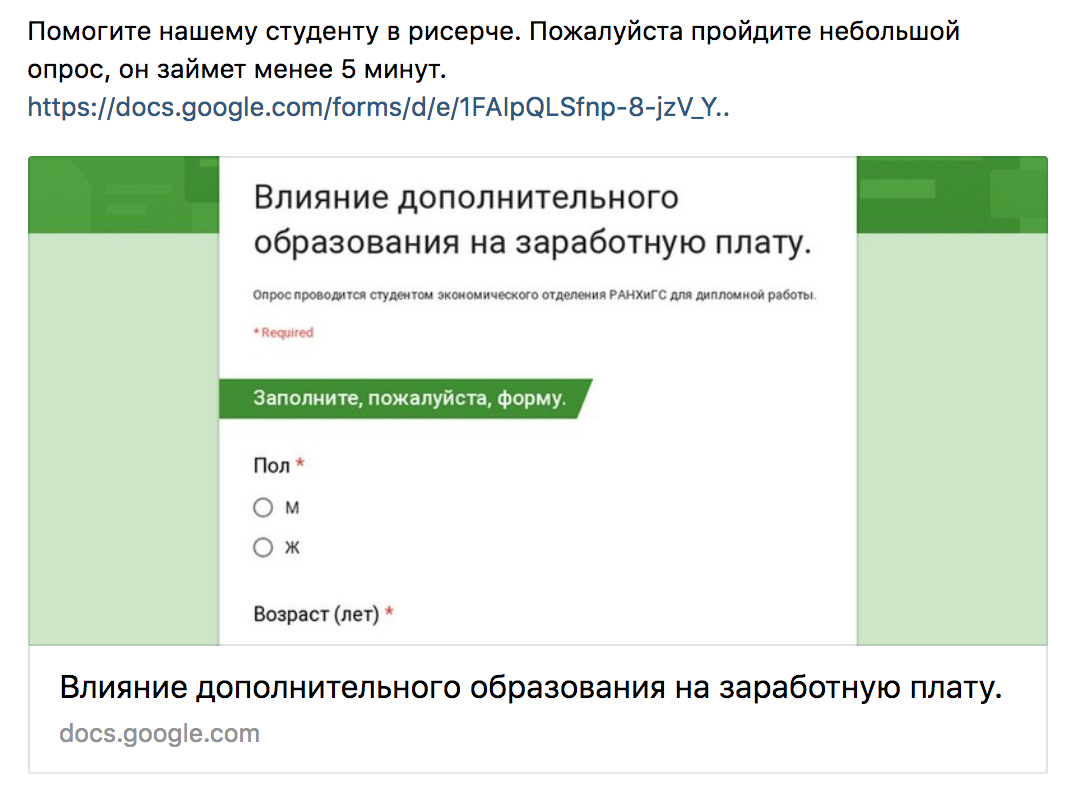
\includegraphics[scale=0.4]{research.png}
    \caption{Мольба студента-маркетолога о помощи} \label{fig:salary}
    \end{center}
\end{figure}
 
В такой ситуации мы столкнёмся с проблема самоотбора. Человек должен хотеть заполнить анкету. Очень маловероятно, что люди с высокой зарплатой решат потратить своё время на заполнение анкеты. Их время слишком дорого стоит. В итог, в исследовании о влиянии образования на зарплату будут сделаны неправильные выводы.  


\subsection{Правда ли, что вы гей?}

Другой пример --- опросы, которые связаны с разными чувствительными темами. Что вы ответите интервьюеру, если он на улице спросит у вас, курили ли вы марихуану? Скорее всего, вы либо откажитесь отвечать, либо соврёте. В результате социологи получат некорректную статистику. 

В 2010 году Британское управление национальной статистики (Office for National Statistic, ONS) опубликовало результаты своего исследования о том, сколько взрослых британцев являются геями\footnote{Часть примеров позаимствованы отсюда: \url{https://www.profmatt.com/are-you-gay}}. Опросы показали, что это примерно $1.5\%$\footnote{\url{https://www.theguardian.com/world/2010/sep/23/gay-bisexual-population-uk}}. При этом исследование Кинси конца 1940-х указывало цифру около $10\%$\footnote{\url{https://en.wikipedia.org/wiki/Kinsey_Reports}}. Общепринятым мнением было, что в наши дни эта цифра находится в районе $5-7\%$. И кому верить? 

Проблема нового опроса заключалась в том, что только $96\%$ респондентов согласились разговаривать с социологами. Оставшиеся $4\%$ не стали отвечать на вопрос о своей сексуальной ориентации. Возможно, что они были геями и не хотели в этом признаваться исследователям. Если бы это было так, то доля геев подскочила бы до $5.5\%,$ величины которая находится в пределах ранее полученного диапазона. Конечно же, мы не можем знать наверняка, что это так. Возможно, что отказы отвечать связаны с чем-то другим. Также вполне может быть, что часть респондентов соврала о своей сексуальной ориентации. 

А важна ли вообще эта цифра? На самом деле да. Например, правительство Тони Блэра в Британии при разработке своей социальной политики опиралось на цифру в $5-7\%.$ Если бы к нему на стол попала цифра в $1.5\%,$ политика могла бы быть совсем иной. 

Чтобы избежать подобных искажений приходится придумывать разные более хитрые техники исследования. Такие, чтобы респонденты были уверенны, что они в безопасности. Например, можно поступить следующим образом.

\begin{enumerate} 
    \item[1)] Каждому респонденту мы даём монетку, кубик и листок бумаги. 
    \item[2)] Респондент уходит в отдельную комнату. Там он подкидывает монетку и кубик. 
    \item[3)] Если на монетке выпал орёл, респондент честно пишет на бумаге ответ на вопрос <<Правда ли, что вы гей?>>
    \item[4)] Если на монетке выпала решка, респондент честно пишет на бумаге ответ на вопрос <<Правда ли, что на кубике выпало чётноё число?>>
    \item[5)] Листок бумаги сдаётся экспериментатору. Он видит только ответ <<да>> либо <<нет>>, и не знает на какой вопрос он дан. Если респондент гей и боится признаться в этом, он может сказать, что отвечал на вопрос про кубик. Никто не сможет это проверить. 
\end{enumerate} 

Процедура вполне понятна. Не очень понятно, как можно проинтепретировать полученные результаты. На помощь в этом приходит теория вероятностей. Отталкиваясь от неё, можно очистить данные от случайности.

В среднем около половины респондентов будет отвечать на вопрос про сексуальную ориентацию. Вторая половина будет отвечать на вопрос про кубик. У половины кубик выпадет чётной стороной. Получается, что четверть всех ответов точно будет <<да>>. Если процент ответов <<да>> превышает четверть, то превышение должно быть связано с тем, что респонденты ответили <<да>> на вопрос <<Правда ли, что вы гей?>>.

Например, предположим, что есть $100$ респондентов, и $30$ из них говорят <<да>>. Тогда, в среднем, $25$ из них говорят <<да>> из-за того, что у них выпало чётное число. Остальные $5$ говорят <<да>>, потому что они геи.  Поскольку на вопрос <<Правда ли, что вы гей?>> отвечали только $50$ из $100$ респондентов, мы делаем вывод что $5$ из $50$, то есть $10\%$ геи.  

Конечно же, эти цифры приблизительны, но при большом числе респондентов, они будут довольно устойчивыми. Позже мы узнаем с вами о законе больших чисел, который обеспечивает эту устойчивость. В опросе управления национальной статистики участвовало $450 000$ человек. Если бы они использовали эту методологию, их результаты имели бы гораздо более высокую степень достоверности.


\subsection{Самолёты, дельфины и ошибка выжевшего}

Во время Второй Мировой войны американские военные собирали статистику попаданий пуль в фюзеляж самолёта. По самолётам, вернувшимся из полёта на базу, была составлена карта повреждений среднестатистического самолёта.  Военные собирались укрепить дырявые части бронёй. Так бы и поступили, если бы не вмешался статистик  Абрахам Вальд. Как думаете, что он сказал военным и почему? 


\begin{figure}[H]
\begin{center}
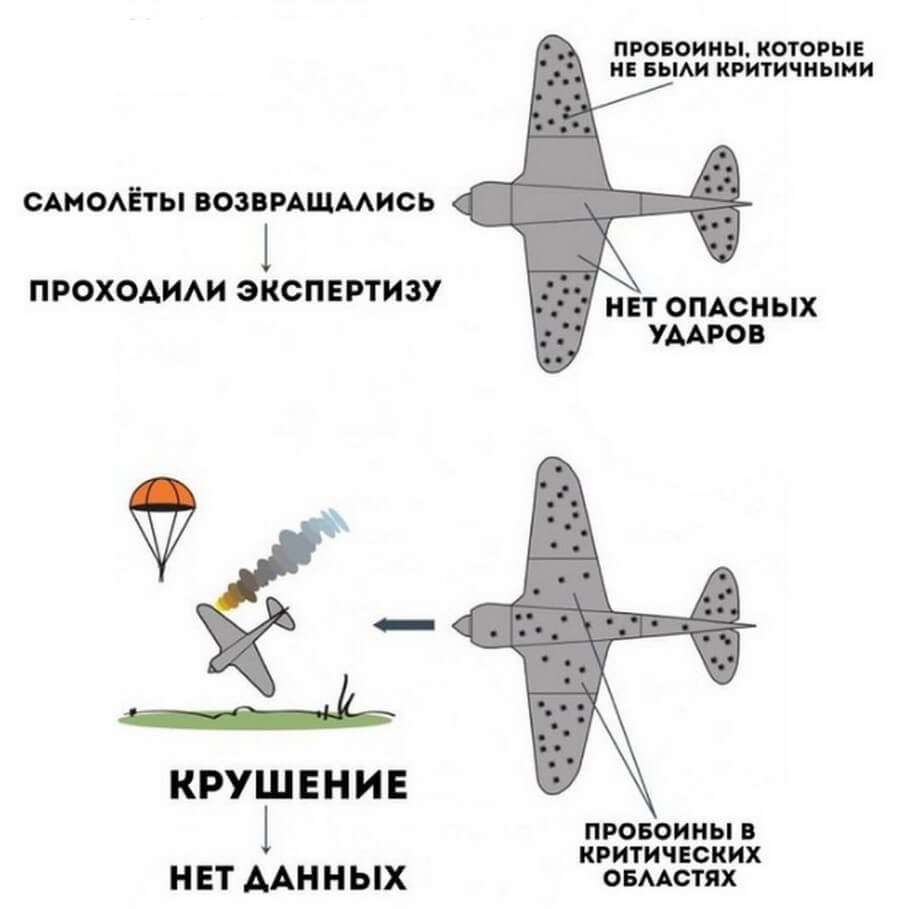
\includegraphics[scale=0.41]{vald_003.jpg}
\caption{Ошибка выжевшего и самолёты Вальда} \label{fig:plane}
\end{center}
\end{figure}

Вальд указал на то, что простреленные части самолёта --- это не его слабые места. Самолёты с критическими повреждениями не возвращаются на аэродром. Поэтому укреплять надо те зоны, где пробоин нет. Если вы хотели укрепить части с пробоинами, вы совершили \indef{ошибку выжевшего.} Это одна из разновидностей ошибки отбора. Она довольно часто мешает делать корректные выводы. Например, все знают, что иногда дельфины выносят на берег людей, потерпевших кораблекрушение. Какие же они умные и дружелюбные! 

На самом деле, дельфины просто любят толкать разные предметы носом. Никому не известно, как много утопающих они затолкали ещё глубже в океан. Мы знаем только примеры чудесного спасения, потому что \indef{жертвы дельфинов ничего никому никогда больше не смогут рассказать.}

\subsection{Зефирный тест} 

Страшнее всего напороться на \indef{эндогенность.} Говоря простым языком, не учесть в исследовании какие-то важные факторы и получить из-за этого неправильные выводы. Слышали когда-нибудь про зефирный тест\footnote{Раздел нагло украден из канала Хулиномика, подписывайтесь нанего: \url{https://t.me/hoolinomics}}? Положите перед ребёнком зефир и дайте ему $15$ минут посидеть с ним в полном одиночестве в пустой комнате. Если малыш выдержит и не съест зефир, он получит вторую зефирку. Если с искушением справиться не выйдет --- тогда второй зефирки ему не полагается. 

Впервые тест проводили в 1960-х в Стенфорде. В 1990-е авторы эксперимента изучили повзрослевших зефирных респондентов и заявили, что те, кто в детстве справился с искушением, оказались гораздо успешнее своих сородичей, съевших зефирку.  Начиная с этого момента, зефирные тесты стали модными. В интернете можно найти довольно много видосов с этим тестом \footnote{\url{https://www.youtube.com/watch?v=goZkgVA68iw}}.

Вроде бы понятно и логично: потерпи, чтобы получить набежавшие проценты. Удержи себя от соблазна сейчас, чтобы получить что-то прекрасное в будущем. Прошло время, и зефирный тест опровергли. Оказалось, что  авторы исследования немножечко налажали с репрезентативностью. Во-первых, они отобрали для исследования всего-лишь $90$ детей. Да ещё и всех из детского садика Стэнфорда. Не каждый бедняк может позволить себе такой детский садик. 

Новое исследование Тайлера Уаттса с коллегами блестяще показало, что дело вовсе не в силе воли, а в богатстве, которое в семье либо есть, либо нет. На этот раз ребята проверили гипотезу почти на тысяче детей, собранных из всевозможных слоёв общества. При этом они учли важные факторы, такие как, например, материальное положение семьи и образование родителей.

В итоге новое исследование обнаружило довольно слабое подтверждение базовой гипотезы (что способность откладывать удовольствие приводит к успеху в жизни). Вместо этого вышло, что возможность продержаться до второй зефирки большей частью определяется финансовым положением семьи ребёнка --- и вот оно-то большей частью и объясняет будущие успехи. А вовсе не умение откладывать удовольствие на потом!

Обнаружилось, что среди детей, мамы которых получили высшее образование, не было никакой разницы в дальнейшей успеваемости. А у тех детей, мамы которых не доучились, преимущество «выигравших» объяснялось социальными факторами, а не способностью дождаться вторую зефирку. Как только исследователи принимали во внимание обстановку в доме трёхлетних испытуемых (например, количество книг на полках, или реакцию мам на просьбы детей), широко воспетая способность «откладывать удовольствие на потом» внезапно переставала означать что-то особенное. Самоконтроль, взятый отдельно от всего, не позволяет детям преодолеть пропасть в благосостоянии и социальном окружении.

Если подумать, то результаты знаменитого теста можно объяснить массой причин. Например, жизнь детей из бедных семей не гарантирует им вообще какую-либо еду, не говоря уже о сладостях. В ожидании ведь есть определённый риск. Даже если родители и обещали им что-то вкусненькое на выходных, вполне вероятно, что финансовая необходимость заставит их поменять своё решение, и вместо обещанных чупа-чупсов мама купит домой пачку риса.

А если вы родились в состоятельной семье, то отложить удовольствие на потом вам не составит особого труда. Опыт подскажет, что финансовое положение семьи стабильно, и у родителей есть ресурсы, чтобы выполнить свои обещания. И даже если такой ребёнок не станет дожидаться второго зефира, у него будет шанс получить вместо него что-то вкусное чуть позже.

Исследователи поведенческой экономики из Гарварда и Принстона написали в 2013 году книгу о бедности под названием «Скудность. Почему обладание малым означает так много». Дело в том, что состояние нехватки чего-либо изменяет образ мышления людей. Бедность легко может сподвигнуть человека на сиюминутную награду. Маргиналы просто иначе оценивают то, что им доступно. Другими словами, второй зефир не имеет значения, если ты сомневаешься, что тебе вообще достанется зефир.

Эти выводы намекают на то, что бедняки стараются баловать детей при первой возможности, а состоятельные родители имеют склонность поощрять ребёнка дождаться более жирной награды. Краска для волос или конфеты могут показаться дурацким подарком, но не забывайте о том, что это порой единственное, что может себе позволить семья из Тамбовской области. А нищим детишкам какая-никакая сиюминутная радость заметно улучшит несчастную жизнь. Ведь у них нет никакой гарантии, что завтра случится хоть что-то хорошее.


\section{Детсадовская аналитика} 

Когда людей собеседуют на аналитические позиции, для разминки им периодически накидывают ситуации, в которых с данными произошёл какой-то трэш. Например, в Яндексе на собеседованиях раньше предлагали задачу <<Детсадовская аналитика>>. Сейчас больше не предлагают, так как её засветили на хабре в одном из разборов\footnote{\url{https://habr.com/ru/post/546004/}}. Попробуйте сами накидать вариантов, в чём конкретно тут возникают проблемы, а потом уже читайте решение.

\begin{problem}{}
Журналисты спросили у $20$ детей в одном детском саду, живут ли их родители вместе. Двое детей ответили, что не живут. На следующий день была опубликована статья под заголовком <<Каждая десятая семья с маленькими детьми в нашем городе разведена!>> Почему выводы журналиста могут быть некорректны?
\end{problem}

\begin{sol} 
Проблем тут вагон и маленькая тележка. Давайте перечислим основные.

\begin{itemize} 
    \item Маленькая выборка, оценка журналиста будет неточной. 
    \item С репрезентативностью выборки большие проблемы. Детский садик может находится в неблагополучном районе. Либо наоборот, в благополучном районе. Он в выборке только один. 
    \item Дети могут врать либо не понимать вопроса из-за маленького возраста.
    \item На одну семью в среднем приходится больше одного ребёнка. Оба ребёнка, сказавших что их родители не живут вместе могут относиться к одной и той же семье. Тогда оценка журналиста просаживается в два раза. Более того, в многодетных и однодетных семьях процент разводов может довольно сильно различаться. 
    \item В поле зрения исследователя попадает не вся генеральная совокупность. Есть много благополучных семей, в которых дети не ходят в садик. Из-за этого оценка журналиста будет завышена. 
    \item Сам по себе вопрос журналиста сформулирован некорректно. Что вообще имеется в виду под <<не живут вместе>>? Возможно, что отец находится в командировке. Возможно, что один из родителей погиб. Это нельзя приравнивать к семье в разводе. 
\end{itemize}

На самом деле в методике журналиста можно найти ещё кучу проблем. Подумайте о том, как эти проблемы можно решить. Как бы вы проводили такое исследование на месте журналиста? 
\end{sol} 

\section{Немного про природу случайности}

Человек --- очень плохой генератор случайных чисел. На многих курсах по статистике лектора проводят следующий эксперимент. Студентов просят написать последовательность из $100$ случайных цифр, сгенерированных из их собственных голов. В процессе оказывается, что генерировать случайные последовательности из цифр --- сложно. Поначалу люди пишут свои цифры довольно быстро, но вскоре замедляются. Они начинают думать о том, как сделать так, чтобы последовательность была случайной. Иногда люди сдаются и начинают писать последовательности, которые уже знают. Например, номера телефонов. 

Со мной такой эксперимент проводили на курсе статистики в Яндексовой школе анализа данных, ШАД. Аудитория из сотни человек в течение $10$ минут генерировала случайные последовательности из цифр. Ассистенты перенесли эти последовательности в электронный вид. Затем семинарист сгенерировал сотню случайных последовательностей и обучил классификатор, который практически идеально отделил последовательности, сгенерированные людьми от компьютерных.

Почему так происходит? Давайте взглянем на картинку \ref{pic:random_unifrom}.  Какой из двух наборов точек кажется вам <<более случайным>>\footnote{Идею позаимствовал у Алексея Шаграева: \url{https://habr.com/ru/post/496750/}}?

\begin{figure}[H]
\begin{center}
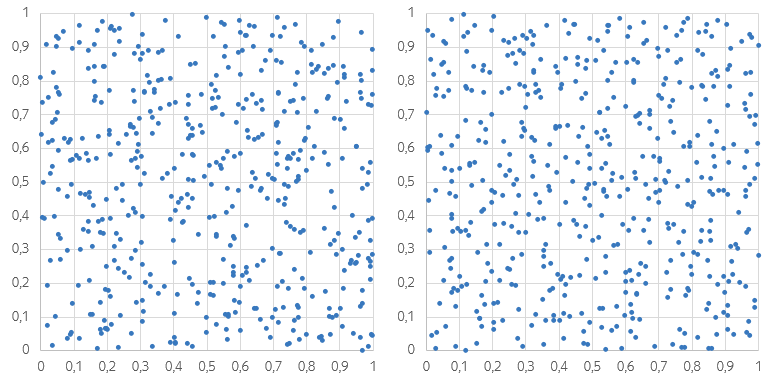
\includegraphics[scale=0.6]{samples.png}
\caption{Случайные выборки}\label{pic:random_unifrom}
\end{center}
\end{figure}

 Выбрали? А вы уверены в своём выборе? Распределение на левом рисунке явно неравномерно. Есть места, в которых точки сгущаются, а есть и такие, в которых точек почти нет: из-за этого даже может показаться, что левый график более тёмный. На правом рисунке локальные сгущения и разрежения тоже присутствуют, но меньше бросаются в глаза.

Меж тем, именно левый график получен при помощи «честного» генератора случайных чисел. Правый график тоже содержит сплошь случайные точки, но эти точки сгенерированы так, чтобы все маленькие квадраты содержали равное количество точек.

Случайность --- очень <<комковатая>> штука. Например, в последовательности $$(1, 6, 4, 8, 8, 2, 0, 9, 1)$$ есть две восьмёрки рядом с друг другом. В списке из $100$ случайных чисел, в среднем, таких двойников будет около десятка. Студенты, как правило, генерируют меньше. Им такие двойники не кажутся случайными. Точно также на картинке выше сгустки из точек показались вам довольно неестественными. 

Люди склонны ассоциировать случайность с равномерностью. Если данных у нас очень много, случайность, действительно, довольно равномерна. Если мы подкидываем монетку $1000$ раз, мы ожидаем увидеть орла примерно в половине случаев.  Однако, в краткосрочной перспективе монетка довольно долго может выпадать орлом. 

Когда на рулетке выпадает красное, все игроки ставят на чёрное. Им кажется, что красное уже выпадало и второй раз этого точно не повториться. При этом, рулетке наплевать на то, что думают люди, а также ей наплевать на свой предыдущий опыт. Каждый бросок делается независимо, и рулетка надолго может <<залипнуть>> на одном из цветов. Такое заблуждение людей в азартных играх называют \indef{ошибкой игрока.}

\begin{center}
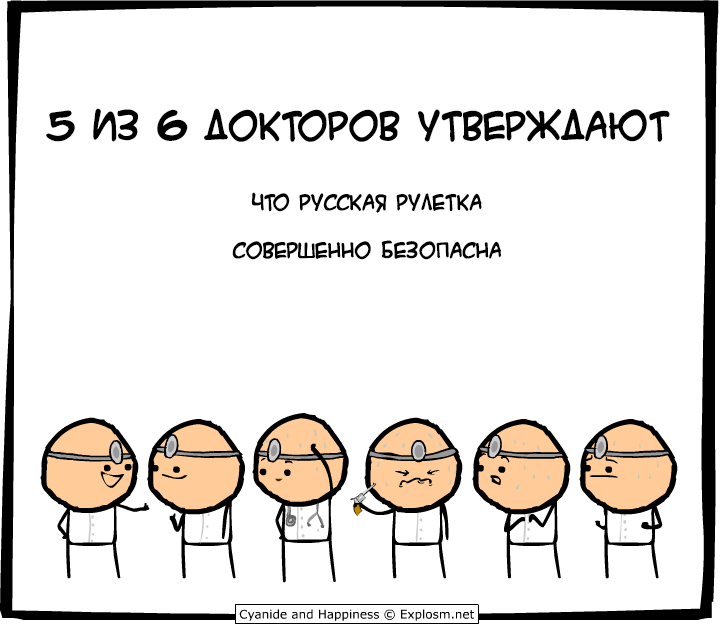
\includegraphics[width=0.5\linewidth]{russian_roll.png}
\end{center}

Эти когнитивные искажения мешают нам жить\footnote{Немного подробнее про то, как именно: \url{https://vas3k.ru/blog/387/}}. Именно из-за них Apple пришлось засунуть в функцию перемешивания в iTunes костыль, который не позволяет включать две песни одного и того же исполнителя друг за другом\footnote{\url{https://www.telegraph.co.uk/technology/11429317/The-biggest-myths-about-technology.html}}. Так последовательность из треков кажется людям более случайной.  


\section{Случайная выборка на практике} 

В реальной жизни сделать честное сэмплирование довольно сложно. Возникает много проблем. Давайте вернёмся к примеру с исследованием зарплаты. Представим себе, что в телефонной книге есть список всех людей, проживающих в Москве. Мы сделали по ней честный сэмпл. Дело осталось за малым --- опросить людей. 

Во-первых, люди могут отказаться с нами разговаривать. Такие люди сделают наш сэмпл непригодным. Мы никак не сможем заменить вывалившегося из него респондента на какого-то нового. Тогда нарушится предпосылка про равновероятное попадание объектов в выборку. Эти вероятность окажутся разными. Более того, такой подход может исказить результаты, как в примере с вопросом <<Правда ли, что вы гей?>>. Тех, кто побоялся ответить <<да>> мы выбросим и заменим на тех, кто твёрдо говорит <<нет>>. 

Вся социология довольно сильно страдает от такой проблемы. Любым цифрам в ней нельзя доверять. Как бы сильно не старались социологи, цифры будут искажены. Поэтому, в социологических опросах люди всегда смотрят на динамику, а не на абсолютные значения. Если был проведён опрос о популярности какого-то политика, и выяснилось, что его поддерживает $60\%$ респондентов --- этой цифре верить нельзя. При этом мы можем делать какие-то выводы по динамике этой цифры. Для этого достаточно каждый месяц проводить опрос каждый месяц по одинаковой методологии и смотреть, падает цифра или растёт. 

Представим себе, что все люди из нашей выборки согласны с нами поговорить. На общение с ними может уйти вечность.  Каждого человека надо найти, от каждого надо выпытать нужную нам информацию. Все живут в разных районах, а кто-то мог вообще уехать из города на время или навсегда. 

Один из способов решить эту проблему --- использовать \indef{кластерную выборку.} Такой подход уместен, когда география нашей генеральной совокупности довольно разнообразна. Мы могли бы попробовать разбить город на кластеры по районам, затем отобрать несколько районов случайным образом, и только после из каждого отобранного района набирать людей. Конечно же, возникает проблема с тем, что вероятности попасть в выборку оказываются для людей разными. Если мы набираем из каждого района по $100$ человек, то в более крупных районах, вероятность попадания в выборку у жителей будет меньше. Однако все эти искажения находятся под нашим контролем и мы можем взвесить на них наши итоговые результаты. 

Другой широко распространённый подход для сэмплирования --- сбор \indef{стратифицированных выборок.} При таком подходе всю генеральную совокупность разбивают на несколько страт и с каждой из них работают независимо. Это помогает улучшить точность статистических результатов.  

Предположим, что мы знаем, что $40\%$ генеральной совокупности составляют мужчины, а $60\%$ женщины. Мы берём случайную выборку из каждой из этих двух групп, страт. Размер каждой выборки делаем пропорциональным её размеру. Например, выборка размера $20$ должна содержать $8$ мужчин и $12$ женщин. Тогда она будет репрезентативной для структуры населения.

Методы стратификации часто используются в онлайн-экспериментах. Предположим, что веб-сервис вносит какие-то изменения в свою работу. Поведение пользователей зависит от характеристик устройств, операционных систем, версий браузеров, характеристик самих пользователей и так далее. Поэтому без стратификации в А/Б-тестах легко столкнуться с тем, что, скажем, доля мобильных пользователей в разбиениях различается на $0.5\%$ и метрики измеряют эффект от этого перекоса, а не от вносимого изменения. Подобного рода ошибки могут портить аналитику и, в конечном счёте, приводить к неверным решениям в развитии продуктов и бизнеса.

Стратифицированный подход в данном случае предписывает разбивать наблюдения на страты (по версиям устройств, ОС, браузеров и т.д.), вычислять метрики внутри страт, взвешивать их сообразно размерам этих страт и таким образом получать значения итоговых показателей. Про это мы будем говорить более подробно в будущих посиделках. 


\begin{thebibliography}{1}
	\bibitem{profmat:ma}
	\emph{Matthew Handy.}
	Probability and statistics a guide for teachers and students at A level and beyond.~//
	\url{https://www.profmatt.com/statistics}.
	
	\bibitem{zhlobolite}
	\emph{Алексей Марков.}
	Жлобология.~//
	\url{https://alexeymarkov.ru/trial/zhlobolite.pdf}.
\end{thebibliography}

\end{document}